\section{The Graphic User Interface}

When launching the GUI, the home screen appears like this :\\


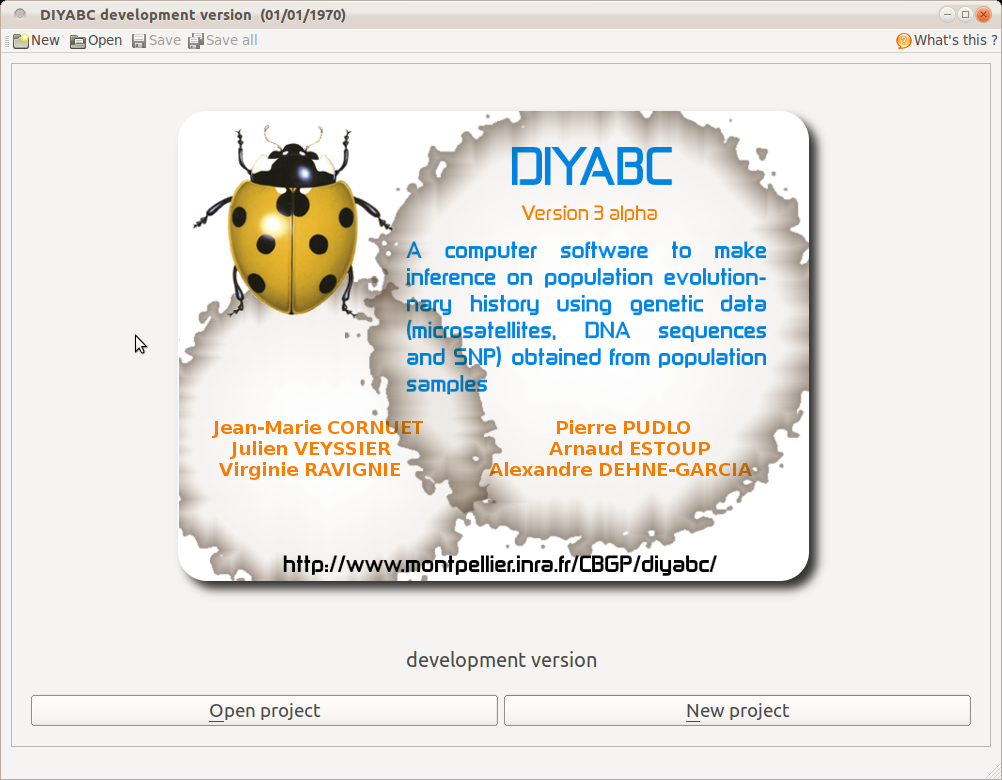
\includegraphics[scale=0.4]{gui_pictures/Capture-DIYABC-1.png} 

You can already notice that $DIYABC$ works with projects. This notion is new to version 2 of $DIYABC$. It is explained in subsection 3.1.

\subsection{What is a $DIYABC$ Project ?}

\label{doc_openProjectButton}
A $DIYABC$ project is a unit of work materialized by a specific and unique directory. A project is defined by at least one observed data set and one reference table header file. These files are located in the \emph{Project directory} which name includes an identifier, the date of creation and a number (between 1 and 100).\\

The header file, always named \texttt{header.txt}, contains all information necessary to compute a reference table associated with the data : i.e. the scenarios, the scenario parameter priors, the characteristics of loci, the loci parameter priors and the summary statistics to compute.
As soon as the first records of the reference table have been saved in the reference table file,  always named \texttt{reftable.bin} and also included in the project directory, the project is "locked". This means that the header file can not be changed anymore. If one needs to change a scenario or a parameter prior, or a summary statistics, a new project needs to be defined. This is to guarantee that all subsequent actions performed on the project are in coherence with the current data and header files. It is of course strongly advised NOT to move files among projects.
Incidentally, the \texttt{header.txt} file is only built when the project has been saved, the information progressively input by the user being saved in a series of temporary files.\\

Once a sufficiently large reference table has been simulated, analyses can be performed. Their different output files are copied to the \emph{analysis} directory included in the project directory, and containing as many directories as analyses performed. Hence, it is now much easier to know with certainty the conditions of each analysis.    

\subsection{Options of the home screen}
The home screen above has three menus and two buttons.\\ 
Let's start with the menus. Below are shown all submenus :

\begin{center} 
\begin{tabular}{ccc}
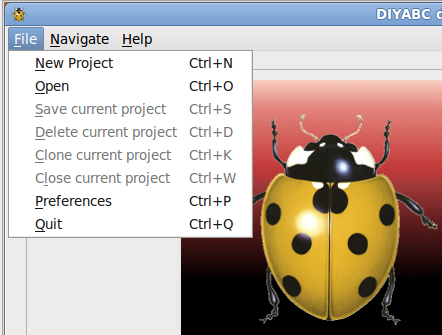
\includegraphics[scale=0.3]{gui_pictures/Capture-DIYABC-2.png} & 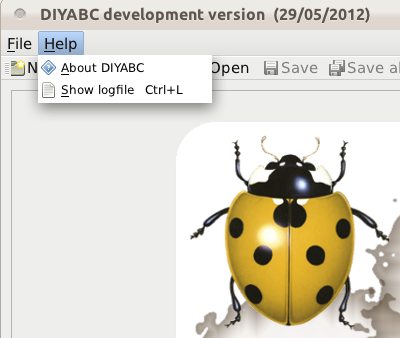
\includegraphics[scale=0.3]{gui_pictures/Capture-DIYABC-3.png}  & 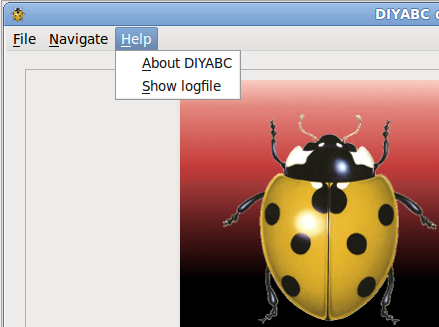
\includegraphics[scale=0.3]{gui_pictures/Capture-DIYABC-4.png}\\
\end{tabular}
\end{center}

The \texttt{File} menu has four active options, namely \texttt{New project}, \texttt{Open project}, \texttt{Preferences} and \texttt{Quit}. All are self explanatory. The first two are redundant with the two buttons. There are also four inactive options that will be active once a project has been loaded or created.\\
The \texttt{Navigate} has two inactive options, \texttt{Next project} and \texttt{Previous project} that will become active once at least two projects have been loaded.\\
The \texttt{Help} buttons has two options, the usual ``about'' giving information on the current version and the authors and a \texttt{Show logfile} which opens up a window showing the list of actions performed by the program.\\
  
Clicking on the \fbox{\textsf{Open project}} button opens up the following frame:\\

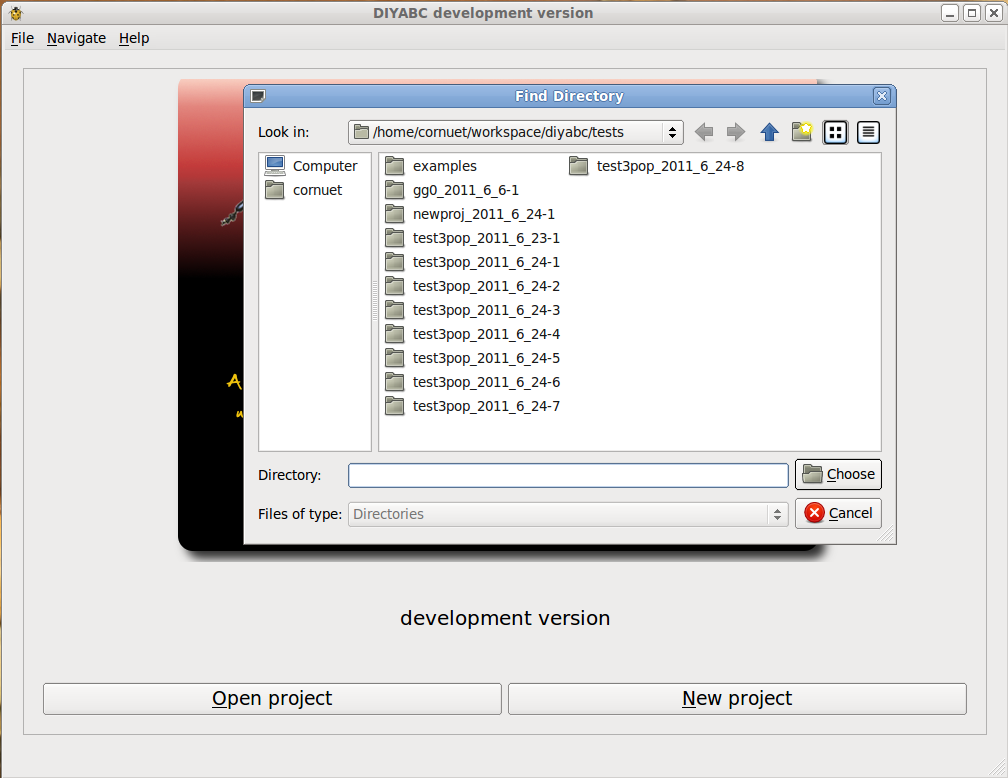
\includegraphics[scale=0.4]{gui_pictures/Capture-DIYABC-5.png} 

To select a project, you just double click on the corresponding directory.
\newpage
 The following screen then appears :\\

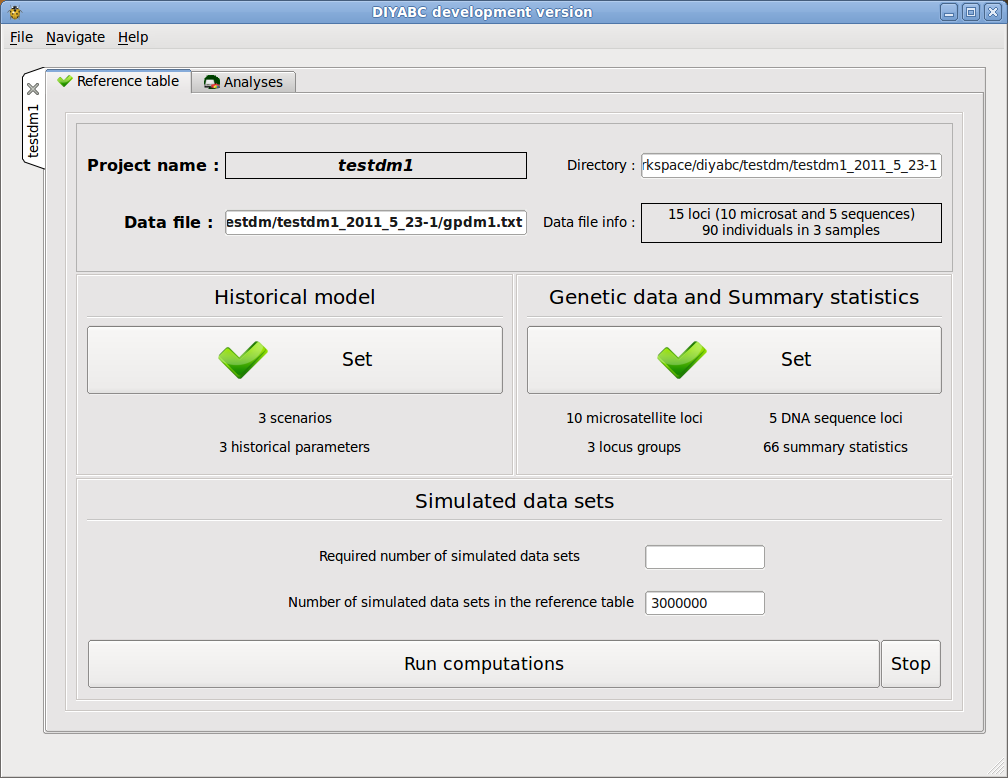
\includegraphics[scale=0.35]{gui_pictures/Capture-DIYABC-6.png} 

We will go back later to the description of this screen.
\begin{itemize}
 \item 
  Cliking on the \fbox{\textsf{New project}} opens up the screen below requiring a name for the new project :\\
\begin{center}
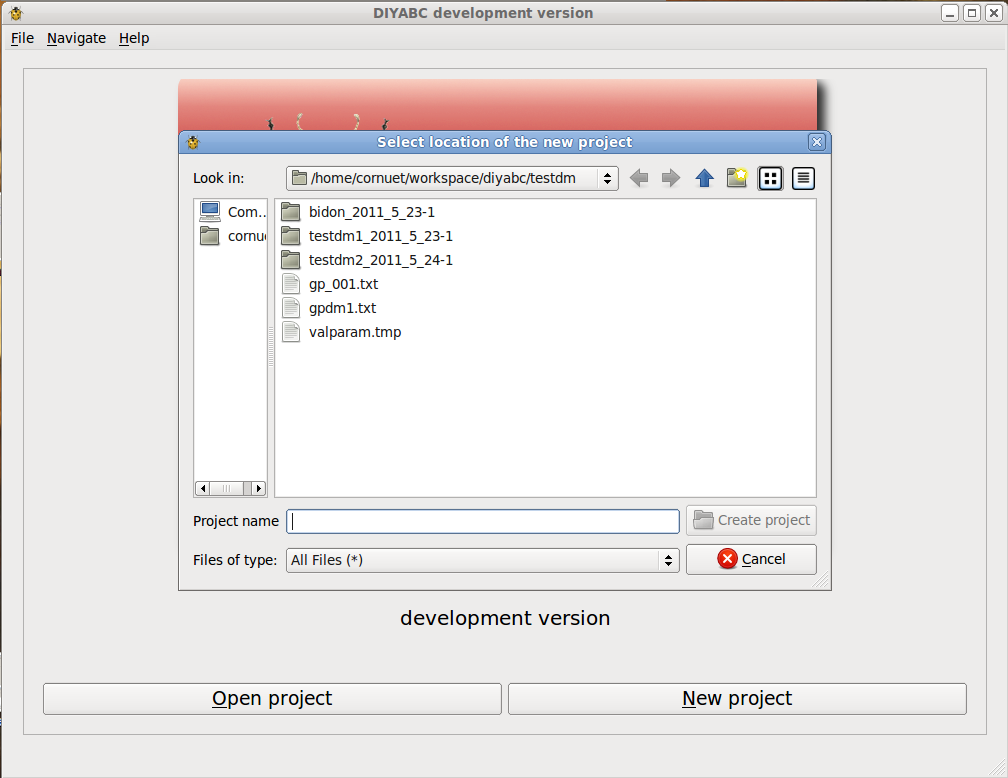
\includegraphics[scale=0.35]{gui_pictures/Capture-DIYABC-7.png} 
\end{center}
\item
After giving a name to new project and cliking on \fbox{\textsf{OK}}, the following screen appears :\\ 

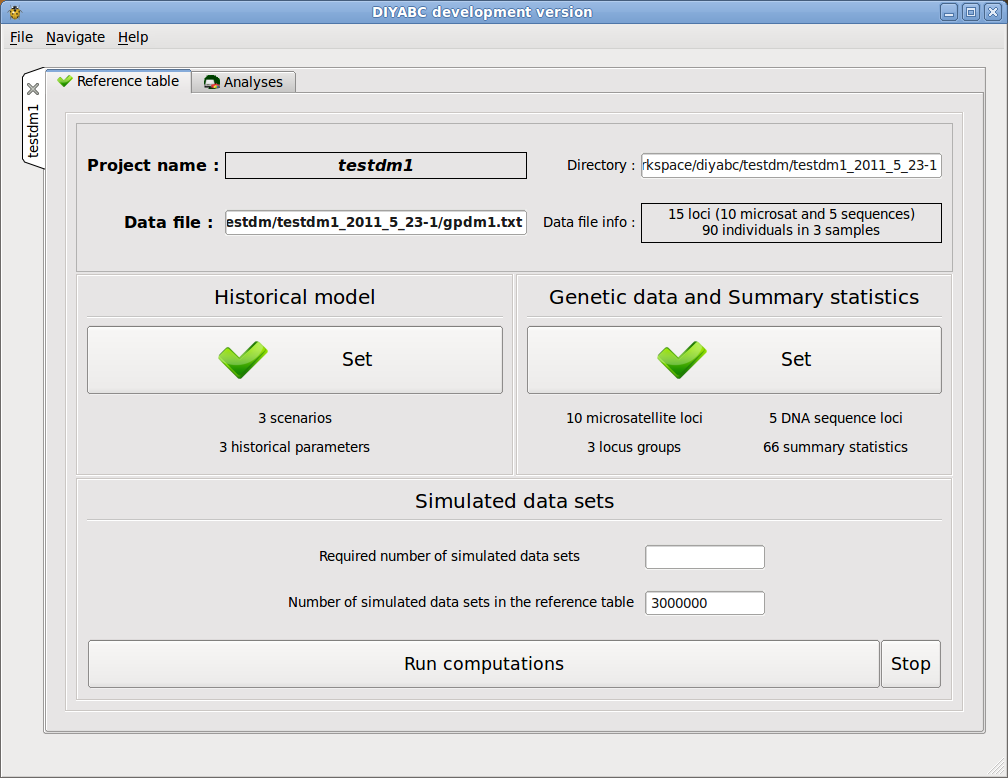
\includegraphics[scale=0.35]{gui_pictures/Capture-DIYABC-6.png} 

\end{itemize}

\subsection{Defining a new project}
Defining a new project requires to follow a number of steps that we are going to detail now.

\subsubsection{Step 1 : choosing the data file}
This is performed by clicking on the corresponding \fbox{\textsf{Browse}} button (previous screen).  The usual file browsing screen appears (below) and one has to select a Genepop format data file, here \texttt{gg\_001.txt}. \\

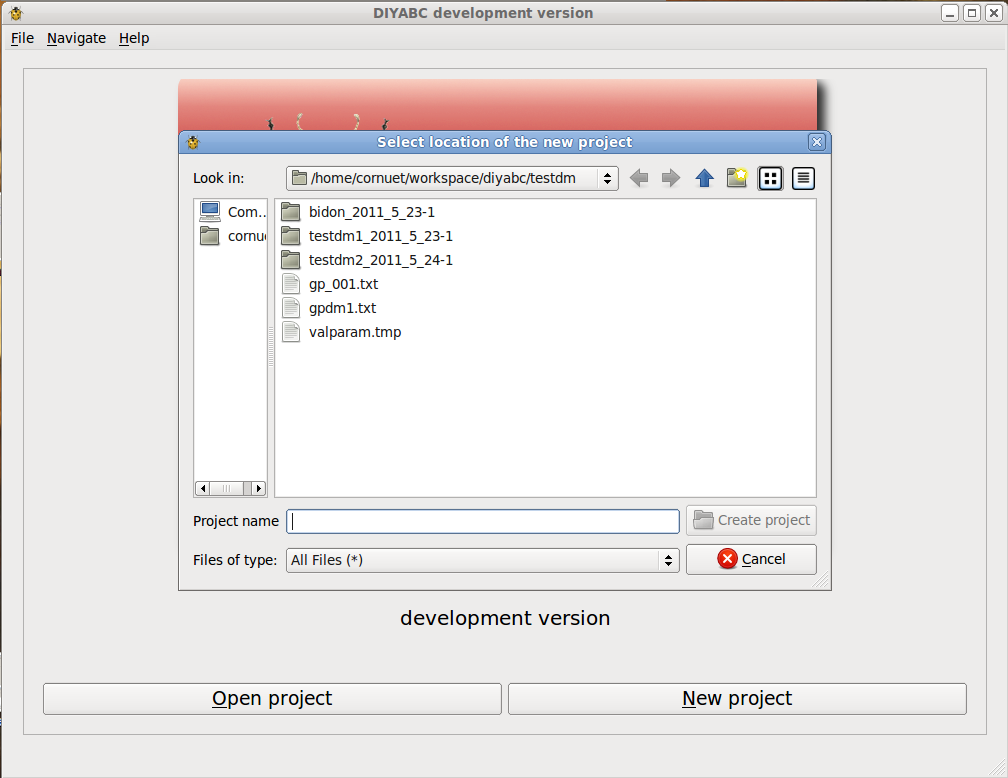
\includegraphics[scale=0.35]{gui_pictures/Capture-DIYABC-7.png} 

Clicking on the \fbox{\textsf{Open}} button leads back to the previous screen with the edit field filled with the name of the data file and some characteristics of this data file appearing on the screen (number of loci, individuals and samples).\\

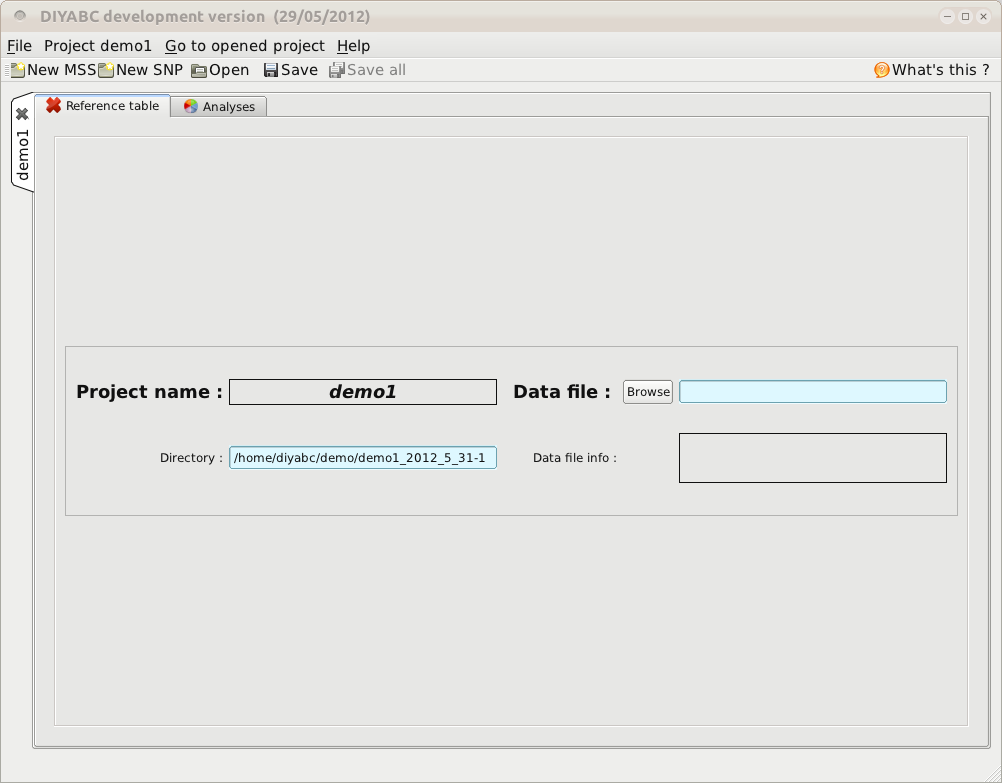
\includegraphics[scale=0.35]{gui_pictures/Capture-DIYABC-8.png} 

\subsubsection{Step 2 : choosing the location of the project directory}
 Click on the corresponding \fbox{\textsf{Browse}} button (previous screen). The usual directory browsing screen appears (below). 
 
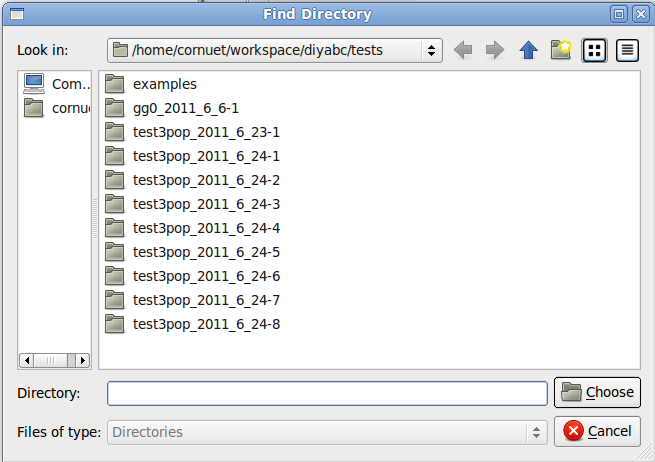
\includegraphics[scale=0.35]{gui_pictures/Capture-DIYABC-9.png} 
 
Clicking on the  \fbox{\textsf{Choose}} button will create the new project directory in the \texttt{/home/cornuet/workspace/diyabc/tests} directory as shown in the screen below.\\  

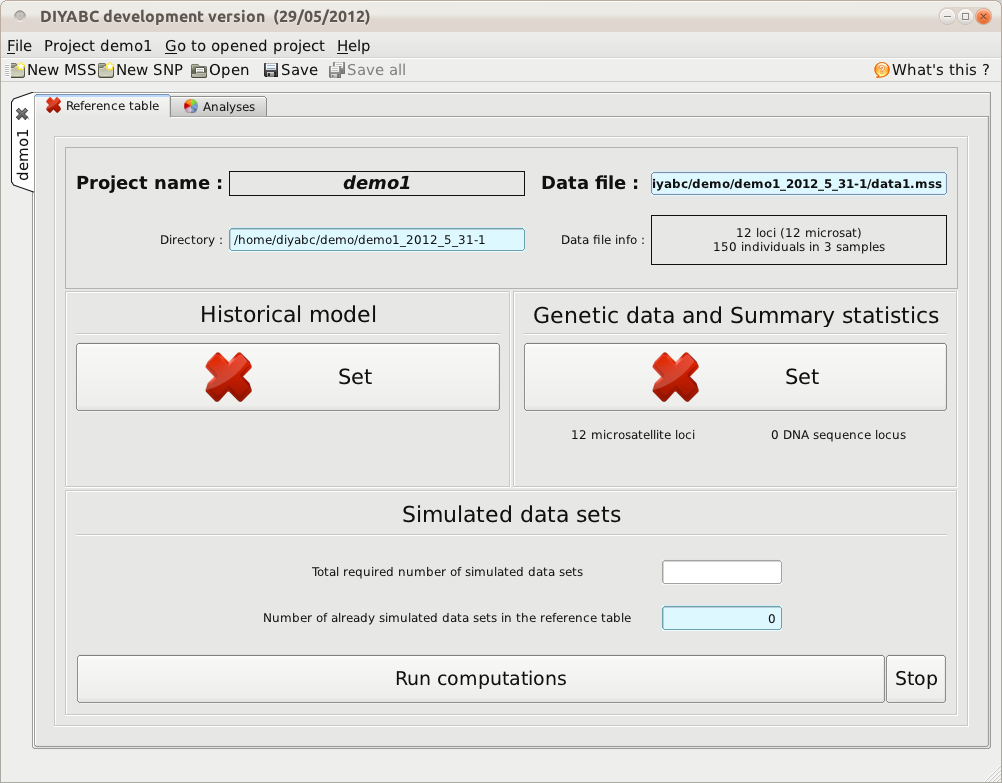
\includegraphics[scale=0.35]{gui_pictures/Capture-DIYABC-10.png} 
 \vfill
 Three new frames have appeared on the screen : Historical model, Genetic data/Summary statistics and Simulated data sets. The first two screens show a red cross meaning that they require information from the user. Once this information will be input and validated, the red cross will change to a green check sign as already shown on page 18.
 
 \newpage
\subsubsection{Inform the Historical model}
Click on the corresponding \fbox{\textsf{Set}} button. The following screen, familiar to users of previous versions, appears:\\

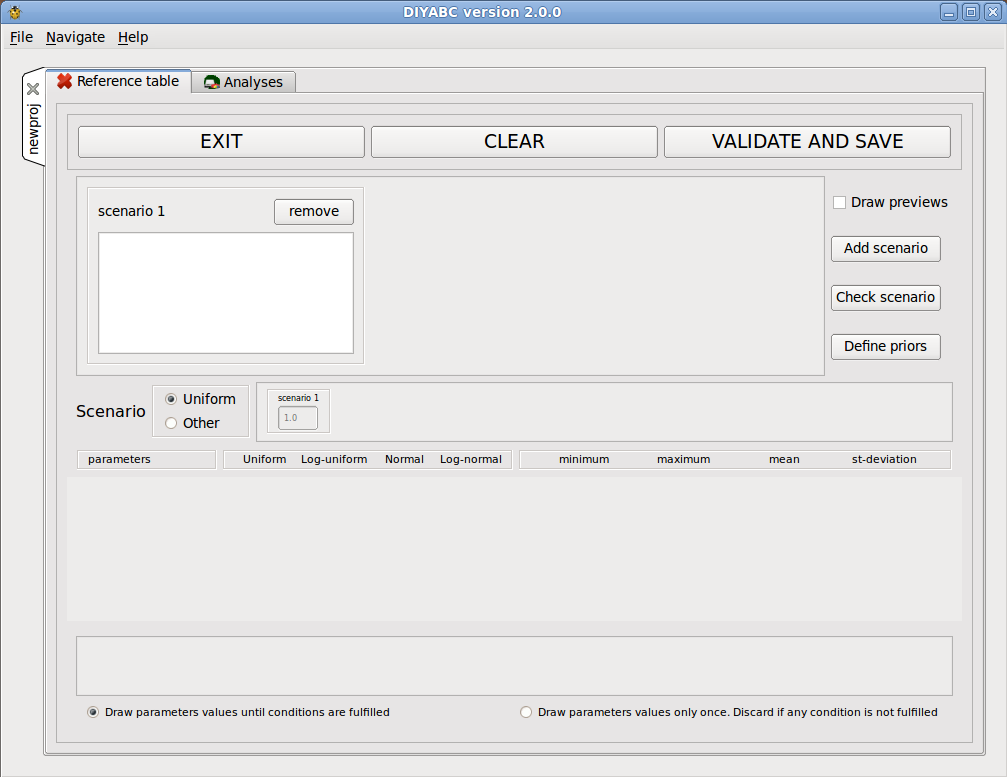
\includegraphics[scale=0.35]{gui_pictures/Capture-DIYABC-11.png} 

Let's enter a simple scenario in scenario 1 edit window and click on the \fbox{\textsf{Define priors}} button. We get this :\\

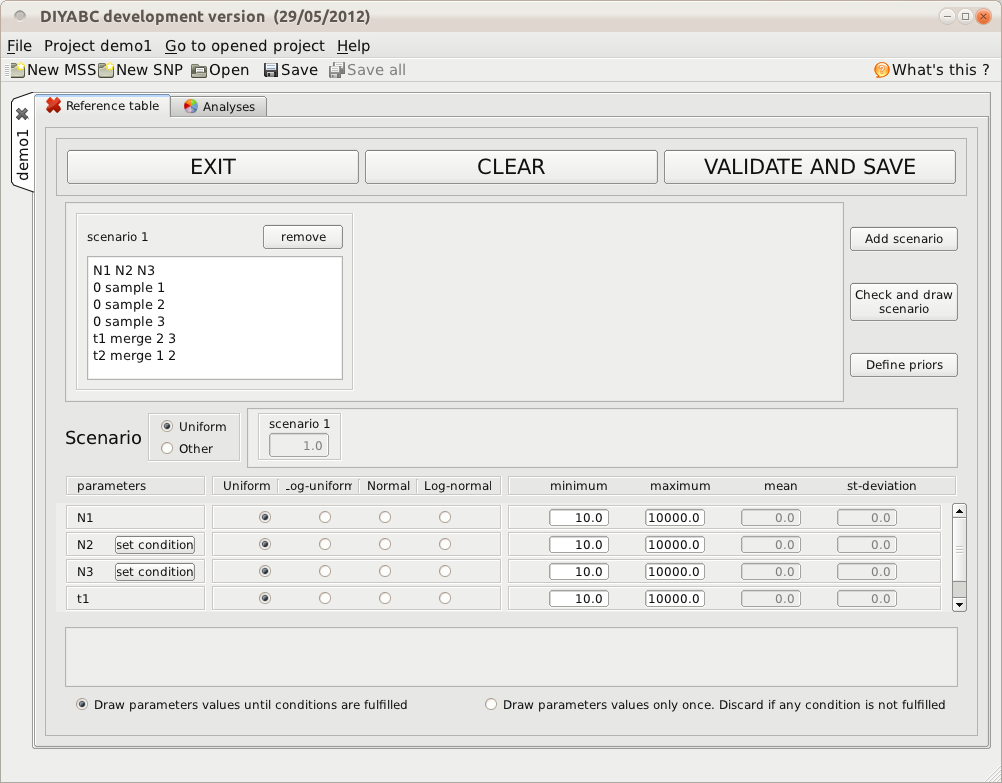
\includegraphics[scale=0.35]{gui_pictures/Capture-DIYABC-12.png} 

The parameter prior frame allows to choose the prior density of each parameter. A parameter is anything in the scenario that is not a keyword (here \texttt{sample,split} and \texttt{merge}), nor a numeric value. In our little scenario, parameters are hence : \texttt{N1, N2, N3, t1, r1} and \texttt{t2}.\\

If we click on the \fbox{\textsf{Check scenario}} button, the logic of the scenario is checked and if it is found OK, and if the scenario is drawable, the drawing appears on a new frame : \\

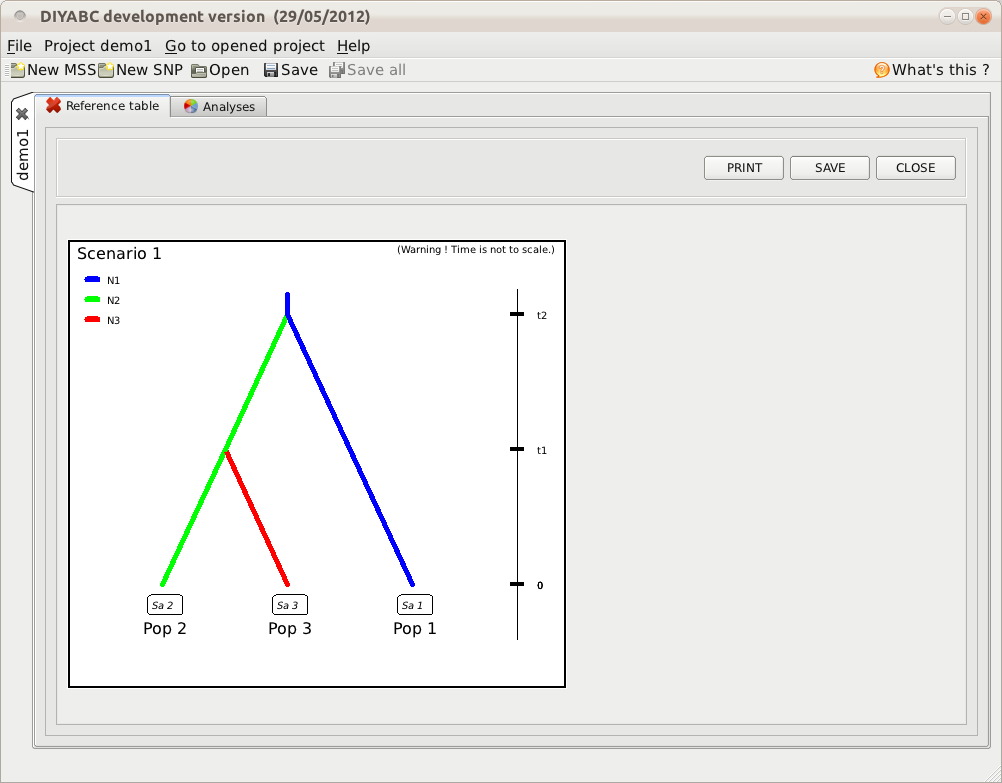
\includegraphics[scale=0.35]{gui_pictures/Capture-DIYABC-13.png} 

The scenario can be saved by clicking on the \fbox{\textsf{SAVE}} button. The frame can be close by clicking on the \fbox{\textsf{CLOSE}} button.\\

Since the scenario has been checked, we can validate and save the historical model by clicking on the  \fbox{\textsf{VALIDATE AND SAVE}} button (bottom screen of p 21). We go then go back to the project screen in which the historical model has now received the green check sign.\\

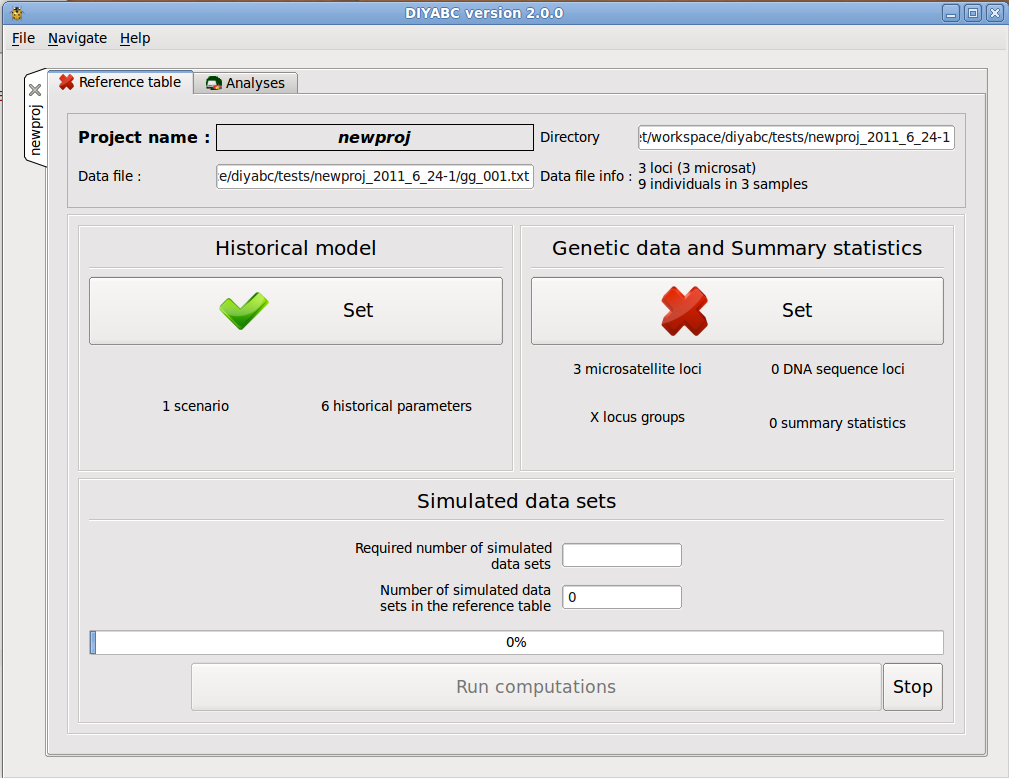
\includegraphics[scale=0.35]{gui_pictures/Capture-DIYABC-14.png} 

 \newpage
\subsubsection{Inform the Genetic model}

Click on the corresponding \fbox{\textsf{Set}} button. We get the following screen : \\

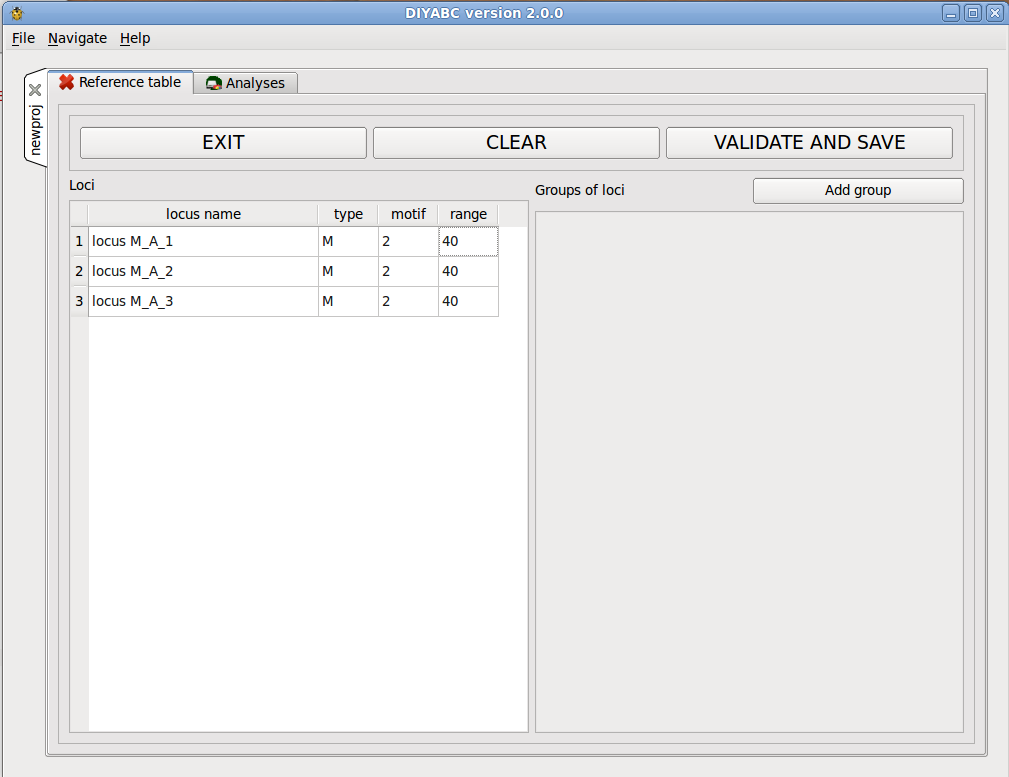
\includegraphics[scale=0.35]{gui_pictures/Capture-DIYABC-15.png} 

On the left part of the screen, there is the list of loci, with their type (M for microsatellites or S for DNA sequences) and the motif size and range for microsatellite loci only. Actually, the values for motif size and range are just default values and do not necessarily correspond to the actual data. The user who knows the real values for its data is required to set the correct values at this stage. If the range is to short to include all observed values, a message appears in a box asking to enlarge the corresponding range. Note that the range is measured in number of motifs, so that a range of 40 for a motif length of 2 bp means that the difference between the smallest and the longest alleles should not exceed 80 bp.\\
We then need to define at least one group of loci by clicking on the \fbox{\textsf{Add group}} button. We get this :\\

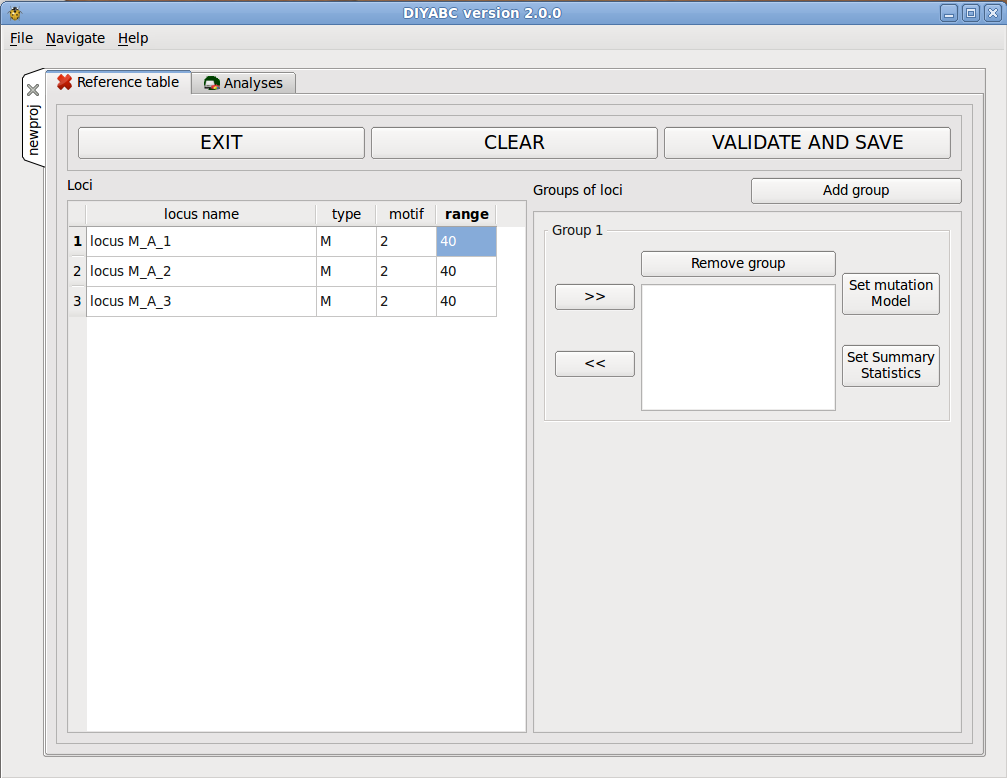
\includegraphics[scale=0.35]{gui_pictures/Capture-DIYABC-16.png} 

Suppose we want the three loci in the same group. We select them like in any table, extending the selection with the \texttt{Shift} and \texttt{Control} keys (see below) : \\

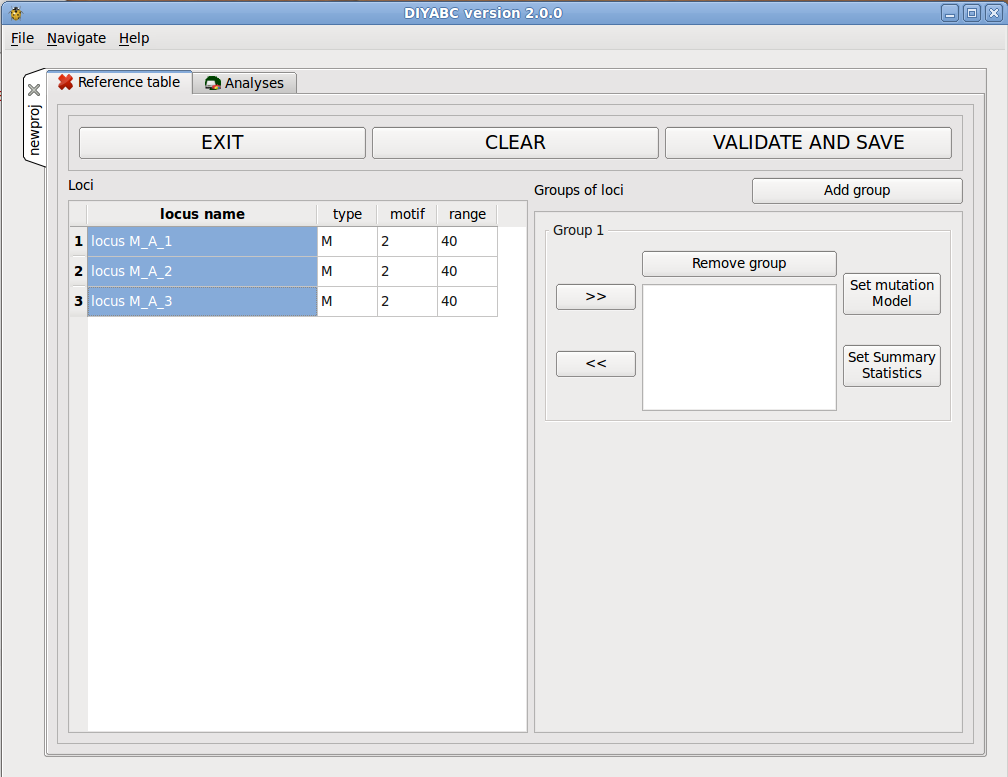
\includegraphics[scale=0.35]{gui_pictures/Capture-DIYABC-17.png} 

and then pressing the \fbox{\textsf{$ >> $}} button : \\

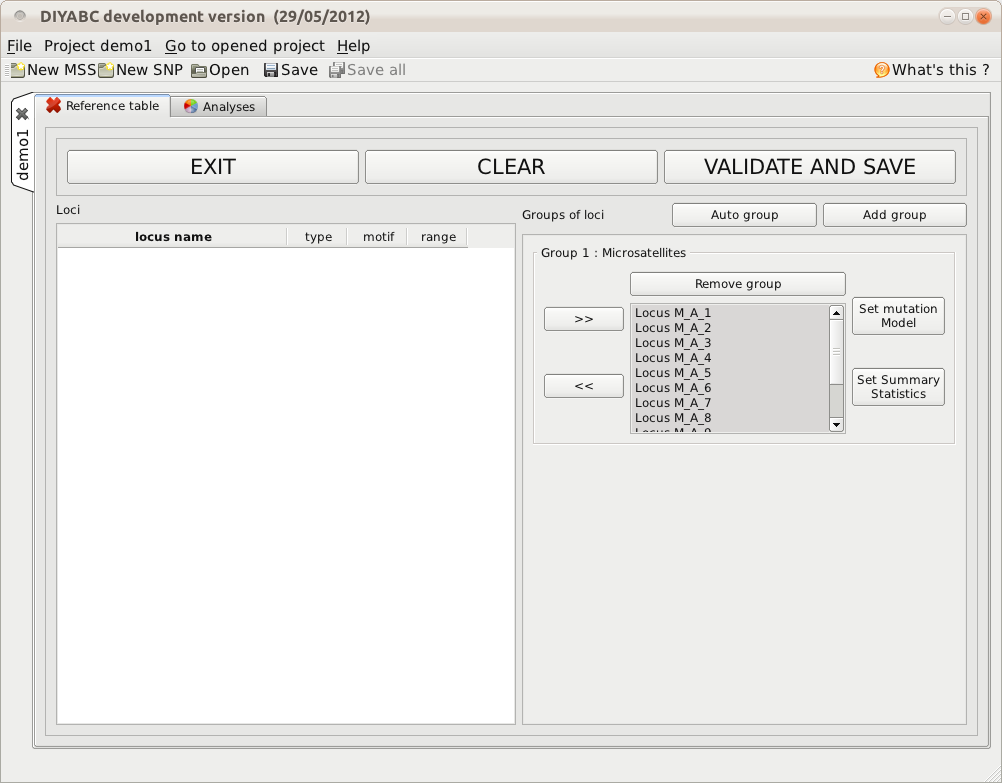
\includegraphics[scale=0.35]{gui_pictures/Capture-DIYABC-18.png} 

We then need to define the mutation model and the summary statistics of the locus group. Clicking on the \fbox{\textsf{Set mutation model}} button, the following screen appears :\\

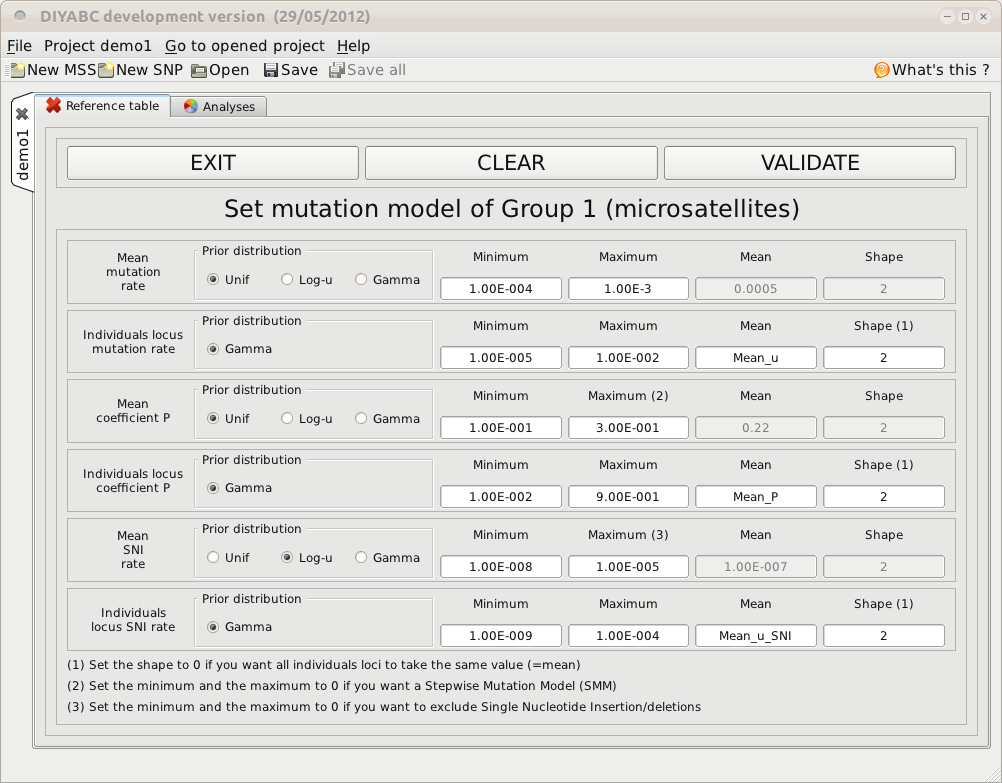
\includegraphics[scale=0.35]{gui_pictures/Capture-DIYABC-19.png} 

Once the mutation model of Group 1 is defined, we click on the \fbox{\textsf{VALIDATE}} button to go back to the previous screen.

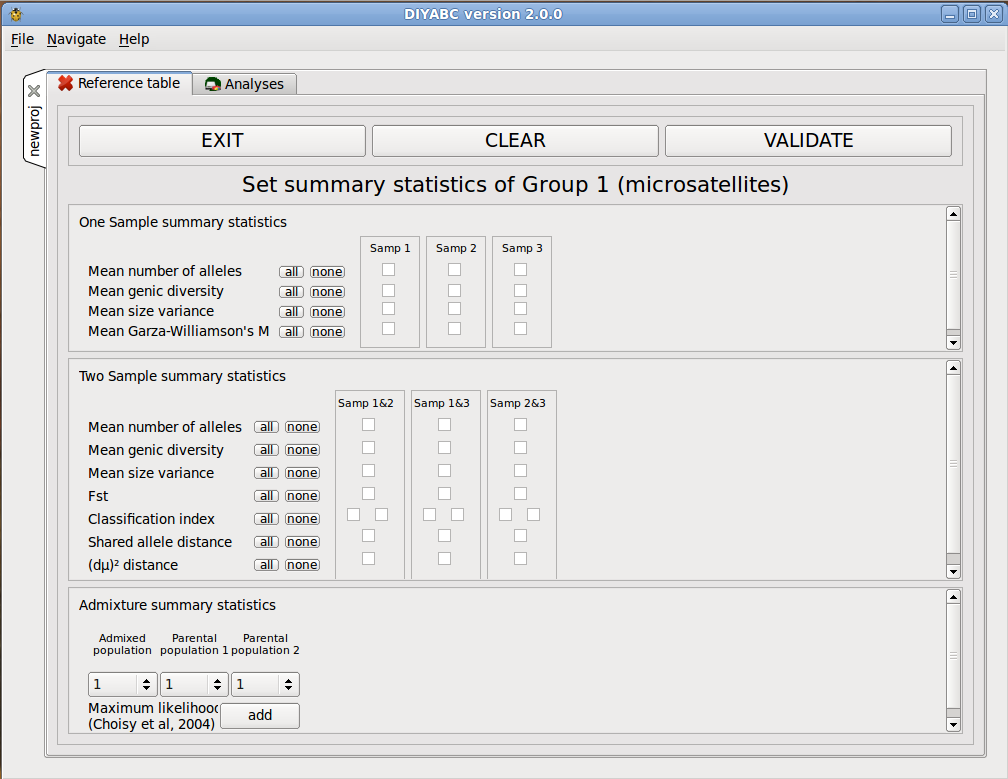
\includegraphics[scale=0.35]{gui_pictures/Capture-DIYABC-20.png} 

We define summary statistics by checking the corresponding boxes :\\ 

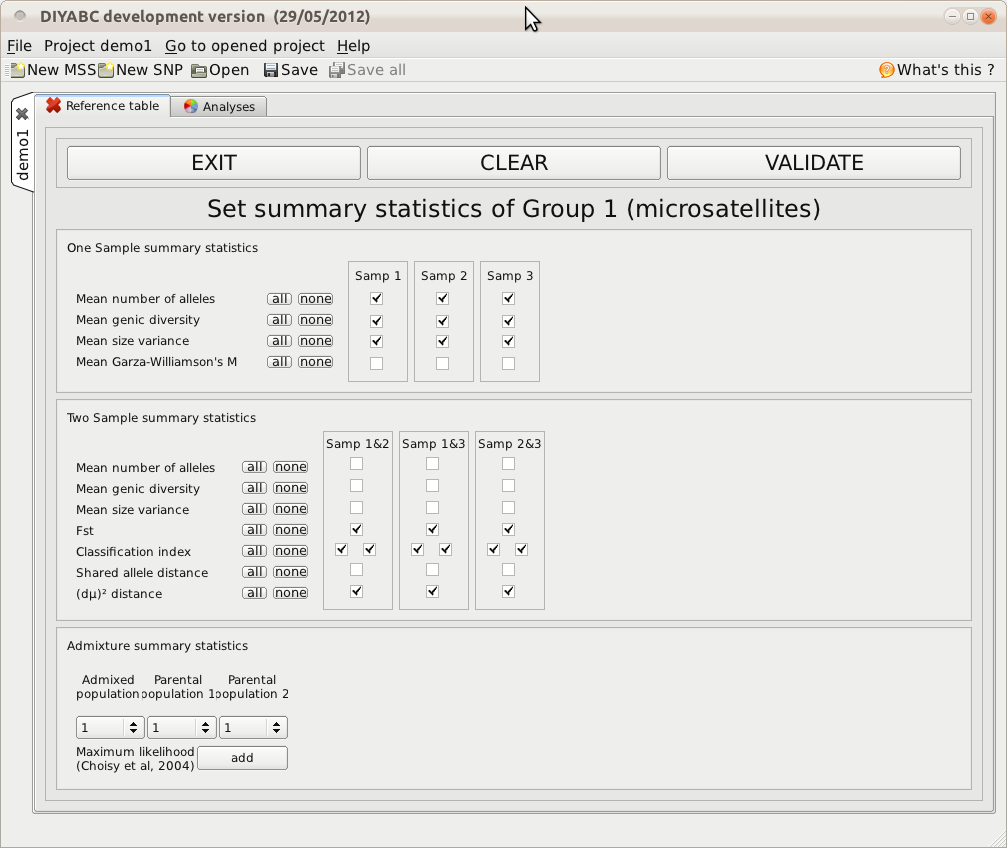
\includegraphics[scale=0.35]{gui_pictures/Capture-DIYABC-21.png} 

Once finished, we click on the \fbox{\textsf{VALIDATE}} button to go back to the screen of p24. Now, we can validate also this screen which brings us back to the screen of p22. The latter looks now like this : \\

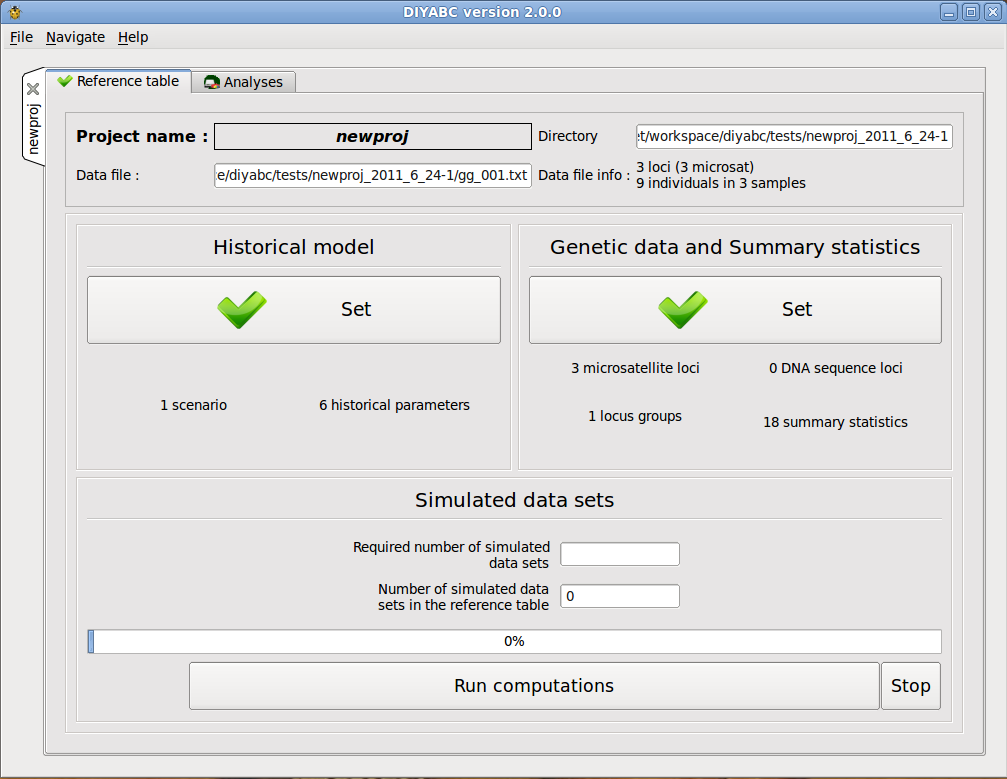
\includegraphics[scale=0.35]{gui_pictures/Capture-DIYABC-22.png} 

At that moment, the project directory includes the following files : a copy of the data file, and four configuration files : \texttt{conf.analysis}, \texttt{conf.gen.tmp}, \texttt{conf.hist.tmp}, \texttt{conf.tmp}. Note that the project is not yet saved. To save the project, we need either to save it explicitly by using the \texttt{File} menu (see below) or to start simulating data sets (next section). Saving the project results in saving the \texttt{header.txt} file in the project directory.


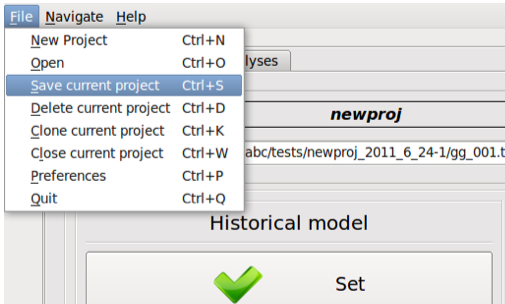
\includegraphics[scale=0.35]{gui_pictures/Capture-DIYABC-23.png} 

\subsection{Building the reference table}

Keeping on the current screen, indicate the required number of data sets to simulate for the reference table : \\ 

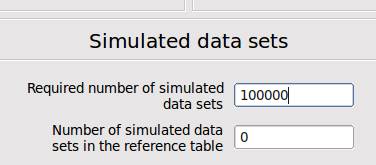
\includegraphics[scale=0.35]{gui_pictures/Capture-DIYABC-24.png} 


Then click on the \fbox{\textsf{Run computations}} button. If things go well, you will soon see the progress both into the edit window "Number of simulated data sets in the reference table" and in the progress bar below. Also, you have an estimate of the remaining time (at the left of the  \fbox{\textsf{Run computations}} button):\\

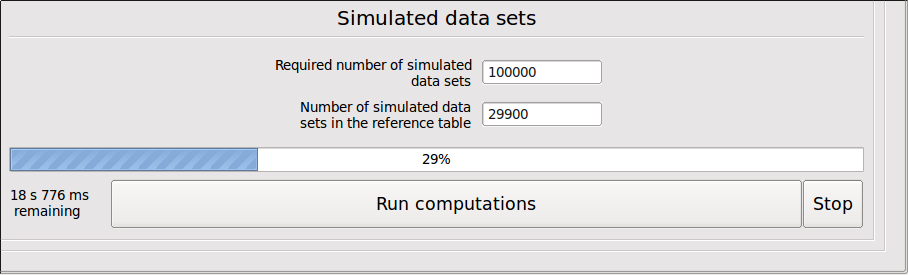
\includegraphics[scale=0.35]{gui_pictures/Capture-DIYABC-25.png} 

When the computation is finished, the screen looks like this :\\

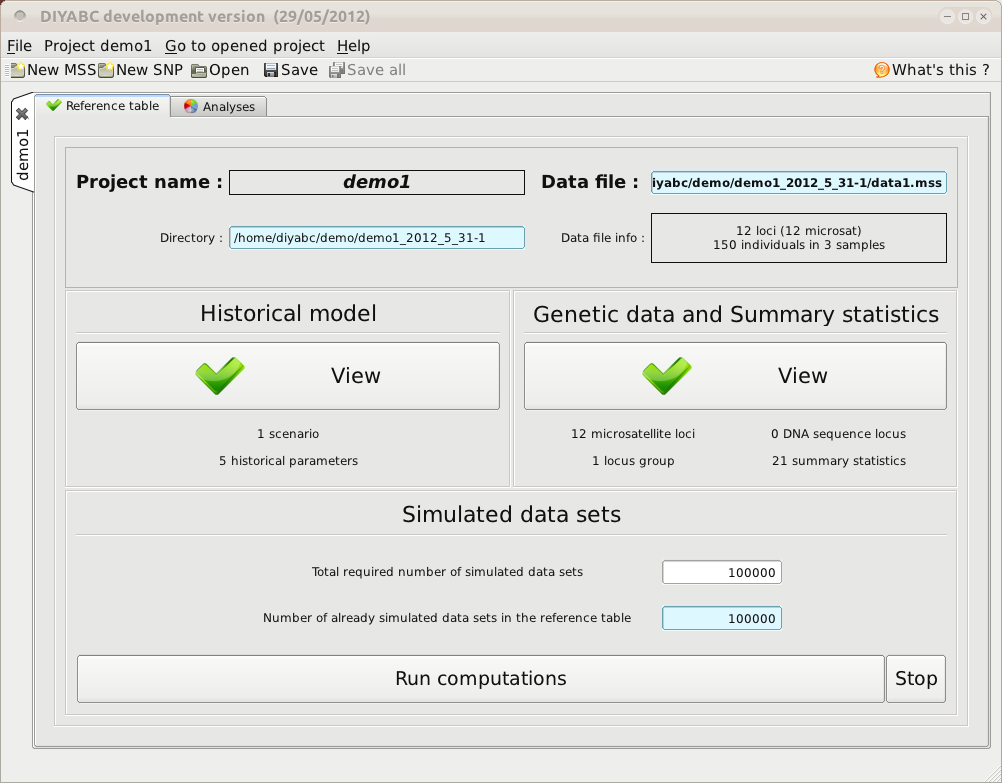
\includegraphics[scale=0.35]{gui_pictures/Capture-DIYABC-26.png} 


\subsection{Defining analyses}
Once the project includes a reference table, analyses can be defined and performed. For that purpose, click on the \texttt{Analyses} tab of the current screen. This shows the following screen:\\
 
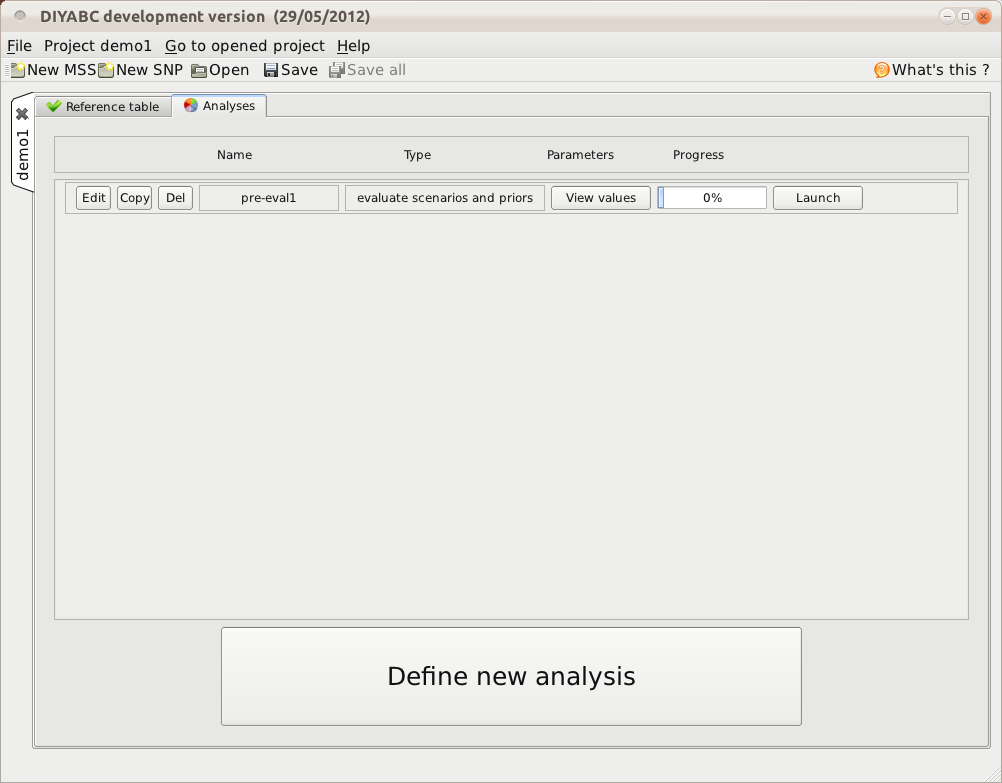
\includegraphics[scale=0.36]{gui_pictures/Capture-DIYABC-30.png} 
 \vspace{20}
We first need to define which kind of analysis we want to perform. So, we click on the \fbox{\textsf{Define new analysis}} button and get this screen:\\ 
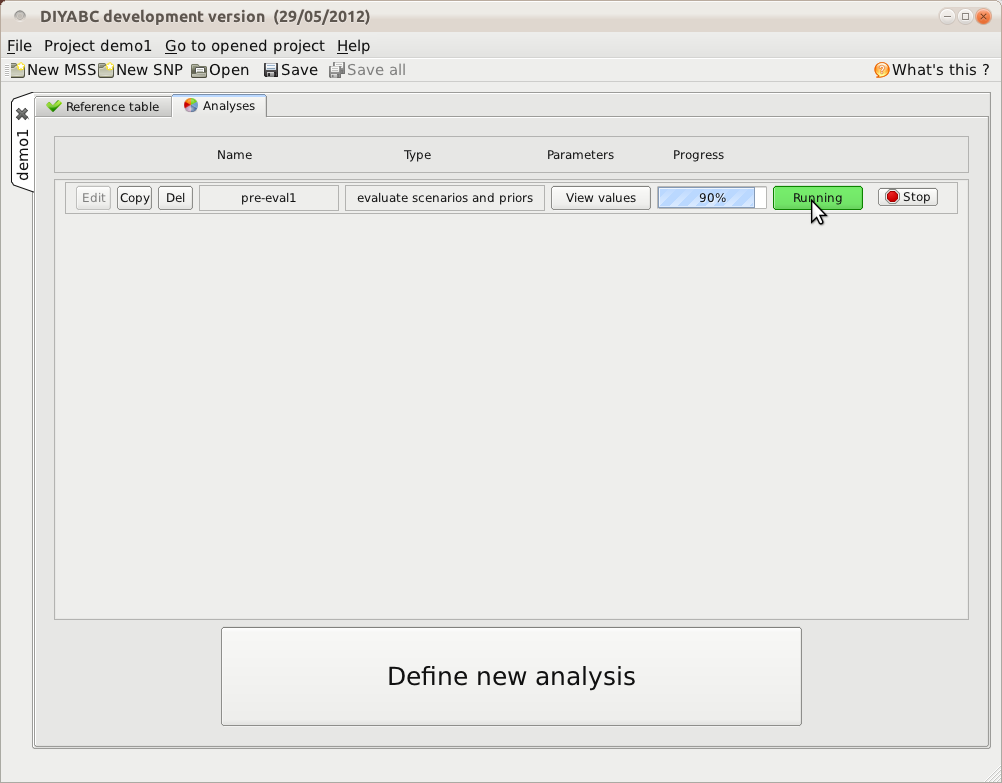
\includegraphics[scale=0.36]{gui_pictures/Capture-DIYABC-31.png} 
 \vspace{20}
The program requires that you give a different name to each analysis that you want to perform.\\
 For instance, we can call the analysis \emph{compar} and choose to compute posterior probabilities of scenarios. We fill the screen accordingly (see screen copy below) and click on the \fbox{\textsf{VALIDATE}} button.\\
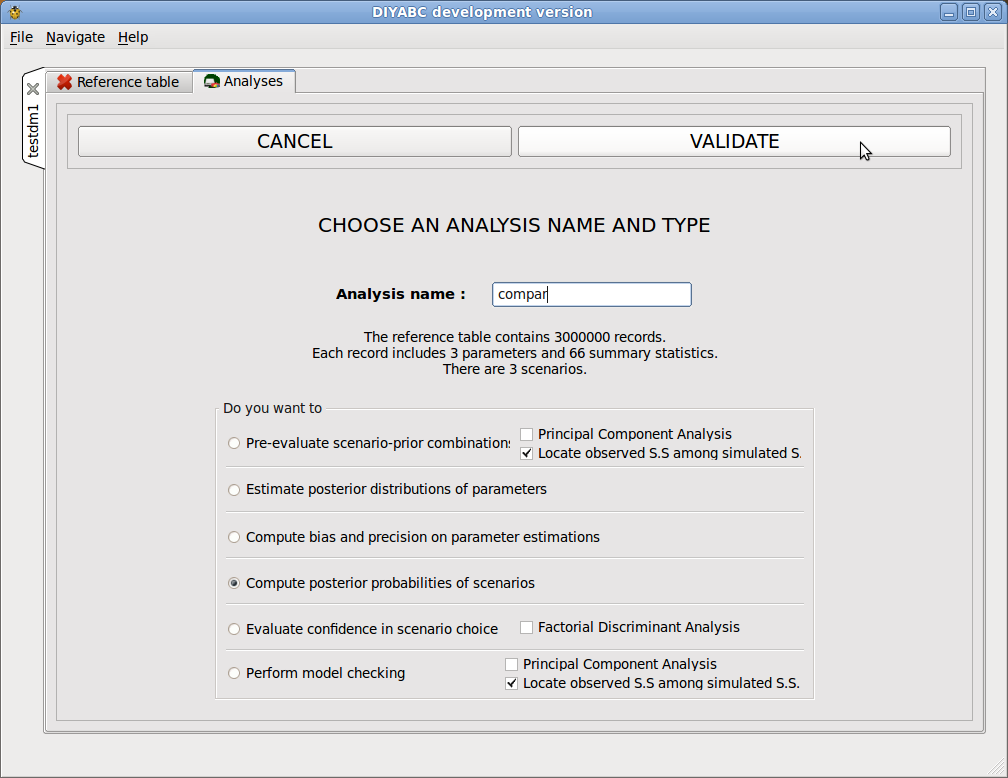
\includegraphics[scale=0.35]{gui_pictures/Capture-DIYABC-32.png} 
 \vspace{20}
Each type of analysis need specific additional information. This will be developed later. Once this information has been given to the program, it goes back to the first Analyses screen:\\
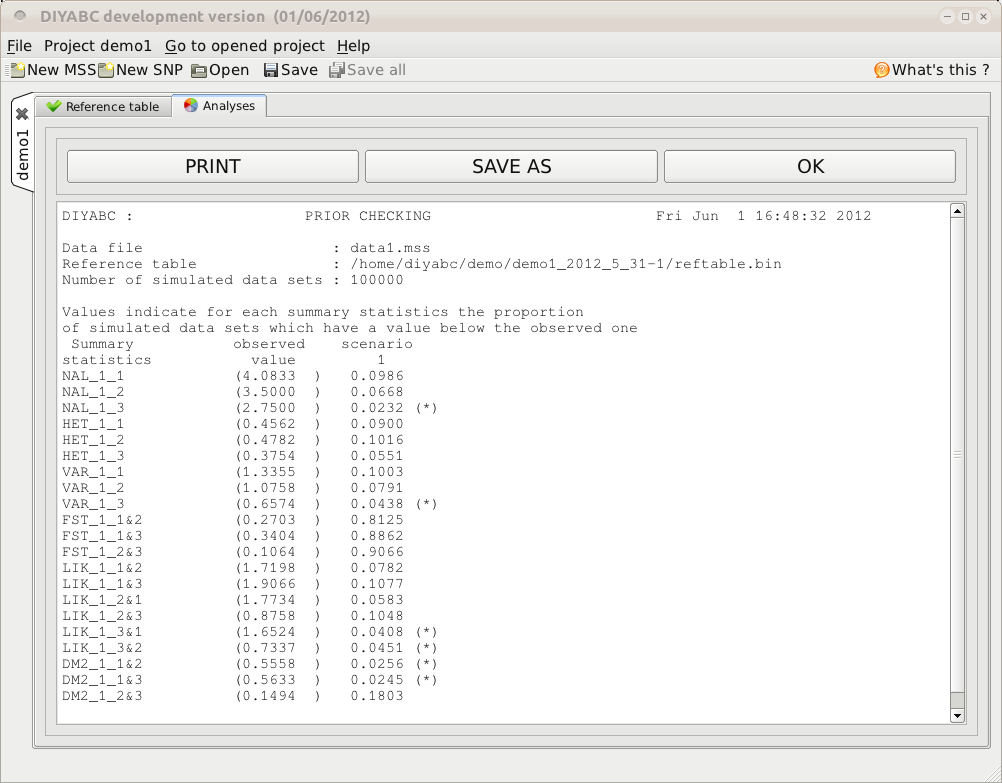
\includegraphics[scale=0.35]{gui_pictures/Capture-DIYABC-33.png} 
 \vspace{20}
This is a kind of dashboard for the set of analyses that you want to perform. You can define all the analyses you need. For instance, in the screen below, five analyses have been programmed :\\
- a comparison of scenarios (\emph{compar})\\
- a pre-evaluation of the combination of scenarios and parameter priors (\emph{preval})\\
- an estimation of parameters under the first scenario (\emph{estim1})\\
- an estimation of parameters under the second scenario (\emph{estim2})\\
- an estimation of parameters under the third scenario (\emph{estim3})\\
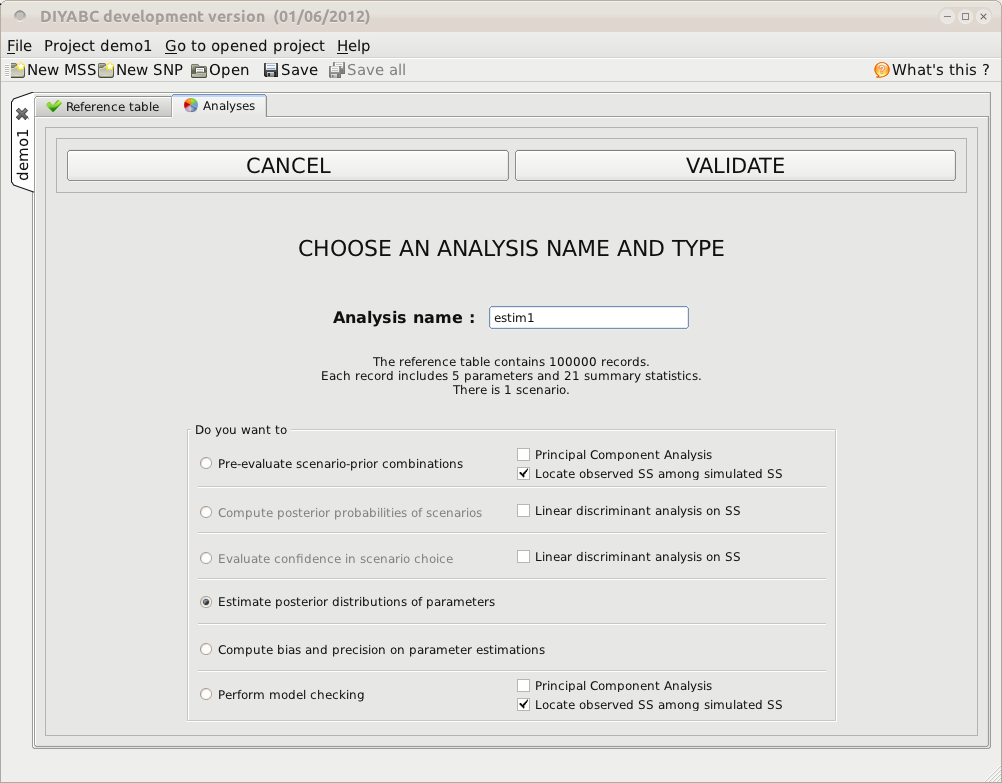
\includegraphics[scale=0.3]{gui_pictures/Capture-DIYABC-34.png} 
 \vspace{20}
Each line of the table corresponds to a single analysis, the name and type of which are given in the corresponding columns. The  
\fbox{\textsf{remove}} button cancels the analysis. The \fbox{\textsf{View values}} show all the information needed for the analysis (see example below). Clicking on the \fbox{\textsf{launch}} button starts the computation only if the computation program is not yet running on this project. If it is yet running, the analysis is put in a queue and will start later. This allows to program a set of analyses and leave the project or the computer while these are running. This can be useful when computation last a long time.
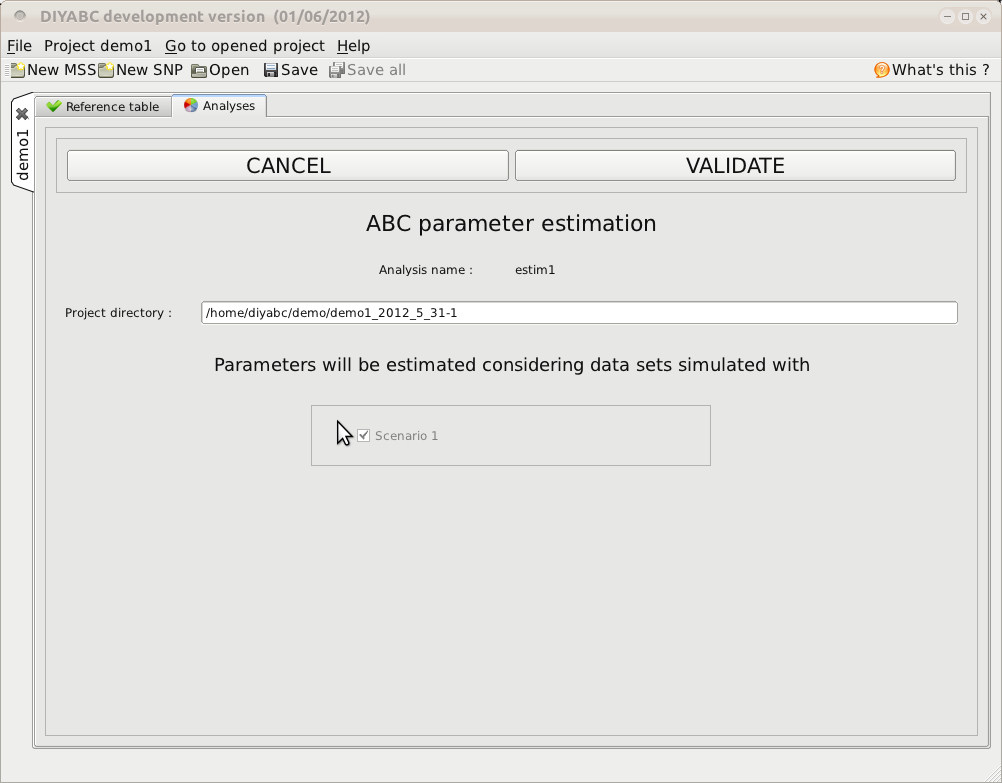
\includegraphics[scale=0.3]{gui_pictures/Capture-DIYABC-35.png} 
 \vspace{20}
The screen below shows a state in which two of the five analysis have been achieved. Notice that for these two analyses, the former \fbox{\textsf{launch}} button shows now a \fbox{\textsf{view}} caption. 
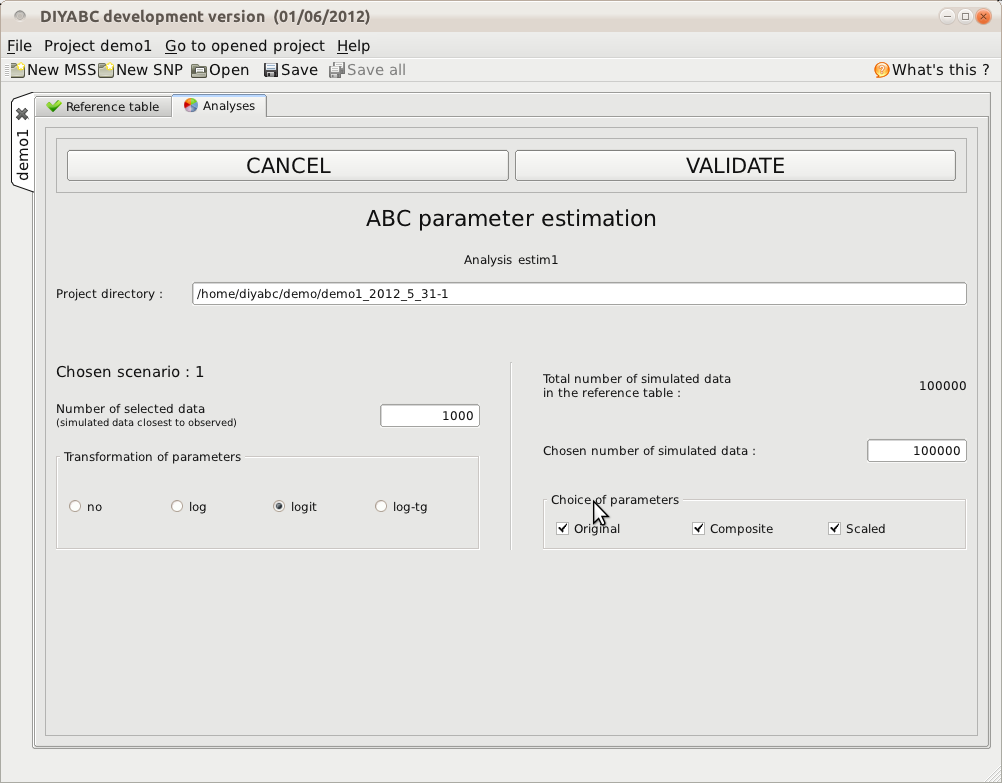
\includegraphics[scale=0.3]{gui_pictures/Capture-DIYABC-36.png} 
 \vspace{20}
Clicking on the \fbox{\textsf{view}} button, e.g. for the \emph{estim1} analysis, gives access to the results of this analysis :\\
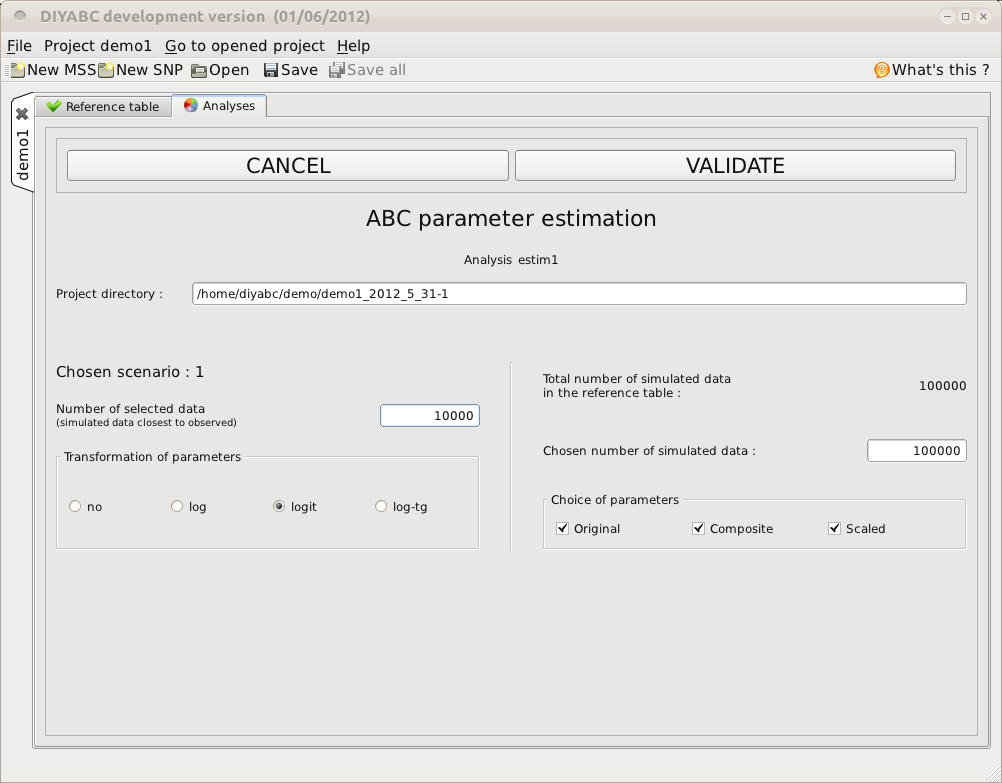
\includegraphics[scale=0.3]{gui_pictures/Capture-DIYABC-37.png}
%\clearpage
